\documentclass[runningheads]{llncs}
\usepackage[T1]{fontenc}

\usepackage[table]{xcolor}

\usepackage{booktabs}
\usepackage[pdfstartview=XYZ,
bookmarks=true,
colorlinks=true,
linkcolor=blue,
urlcolor=blue,
citecolor=blue,
pdftex,
bookmarks=true,
linktocpage=true, % makes the page number as hyperlink in table of content
hyperindex=true
]{hyperref}

\usepackage{rotating} % Rotating table
\usepackage{subcaption}
\usepackage{graphicx}
\usepackage{multirow}
\usepackage{amsmath}
\usepackage{array} % necessary for word wrap within a table



\usepackage{listings} %include R code
\lstset{
    basicstyle=\ttfamily,
    breakatwhitespace=false,         
    breaklines=true,                 
    captionpos=b,                    
    keepspaces=true,                 
    numbers=left,                    
    numbersep=5pt,                  
    showspaces=false,                
    showstringspaces=false,
    showtabs=false,                 
    columns=fullflexible,
    frame=single,
    tabsize=2
}


\title{Buyer Beware: Understanding the trade-off between utility and risk in CART based models using simulation data}
\titlerunning{Buyer Beware}

\author{Jonathan Latner\inst{1}\orcidID{0000-0002-1825-0097} \and
Marcel Neunhoeffer\inst{1,2}\orcidID{0000-0002-9137-5785}  \and
J\"{o}rg Drechsler\inst{1,2,3}\orcidID{0009-0009-5790-3394}}

\authorrunning{Latner et al.}


\institute{Institute for Employment Research, Nuremberg, Germany 
\email{\{jonathan.latner, marcel.neunhoeffer,joerg.drechsler\}@iab.de} \and
Ludwig-Maximilians-Universit\"at, Munich, Germany \and
University of Maryland, College Park, USA
}



\begin{document}

\maketitle 

\begin{abstract}

This study examines the trade-off between utility and privacy when generating synthetic data using Classification and Regression Trees (CART) as a Synthetic Data Generator (SDG). Using low-dimensional simulated data with binary variables, we highlight the limitations of CART in mitigating disclosure risks, demonstrate how common privacy metrics do not capture these risks, and propose parameter modifications to balance the trade-off. Our findings underscore the challenges in identifying privacy risks and the necessity of sacrificing utility to enhance privacy, raising critical questions for synthetic data practices.

\keywords{Synthetic data \and Privacy \and CART \and synthpop}
\end{abstract}

\section{Introduction}

The generation of synthetic data has gained prominence as a means to share data while preserving privacy. It is well-established that there is a trade-off between utility and privacy in synthetic data generation \cite{duncan2004database}. CART models, a widely used synthetic data generator (SDG), are noted for their high utility and relatively low privacy risks compared to other methods \cite{little2022comparing,dankar2021fake}. However, the mechanisms that enable CART to minimize this trade-off remain underexplored.

In this paper, we evaluate whether CART-based SDGs effectively mitigate the risk-utility trade-off.  To do so, we borrow from Reiter et al., \cite{reiter2014bayesian} and simulate a low-dimensional data set with 1000 and four binary variables.  Crucially, the last or 1000$^{th}$ observation is a unique combination of the four binary variables.  In so doing, we create data with an observation we want to protect with synthetic data generated from a CART model.  

In this paper, we seek to make three main contributions.  First, we assess whether we are able to adequately capture the disclosure risks that exist in our simulated data.  Concerns about how to measure utility or privacy in synthetic data are well established.  The problem is not a lack of measures, but rather there is little agreement on which measures are correct for what type of data.  We use common utility and privacy metrics that are available in the Synthpop package \cite{nowok2016synthpop}.  While the results indicate that CART models generate synthetic data with both high levels of utility and privacy, we show that the synthetic data do not protect the disclosive record and this dislosure is not captured by common privacy metrics.  

Second, we explore parameter modifications to the CART-based synthesizer as a potential solution to balance privacy and utility.  On the one hand, we show that one can easily create synthetic data from a CART-based synthesizer that provides a high degree of protection.  On the other hand, we show that one must sacrifice the high levels of utility generated using the default parameters.  Therefore, CART-based synthesizers are capable of generating synthetic data with high levels of privacy protection, but users would have to choose to sacrifice utility even if there is no indication of a disclosure risk.

Third, we propose and evaluate a new implementation of a privacy metric originally developed by Reiter et al., \cite{reiter2014bayesian}. 

<Insert MN text>

In summary, we show that synthetic data from a CART-based SDG are more sensitive to the risk-utility trade-off than was understood from previous research.  Admittedly, we demonstrate this problem using a simulated data set that is unlikely to be used in the real world.  However, the bigger problem is that we demonstrate that there is a disclosure risk in synthetic data that are not captured by common privacy metrics.  If common privacy metrics cannot capture disclosure risks in synthetic data that we know exist (because we created them), then this reduces our confidence that these metrics can capture disclosure risks that we may not know exist.  Although we propose solutions to this problem that operate with low-dimensional data, users interested in generating synthetic data should be aware of the challenges we describe here.

\section{Data and Methods}

Following Reiter et al. \cite{reiter2014bayesian}, we simulate one data set with 1.000 observations and four binary categorical variables.  This is our `original' data set.  The first 999 records were sampled from a multinomial distribution for all combinations of var1(0,1), var2(0,1), var3(0,1), var4(0,1), except the last 1000$^{th}$ record was a unique combination (var1 = 1, var2 = 1, var3 = 1, var4 = 1).  Next, we generate one synthetic data set from a CART-based SDG from the Synthpop package in R with default parameters (seed=1237).  As a sensitivity test, we create 10 synthetic data sets from the original data.


\subsection{Setting up the attack}

The basic idea is that an attack is a game between two entities.  On the one hand, there is a statistical agency who has the data and wants to release them in a way that preserves privacy.  On the other hand, there is an attacker who wants to identify someone in the data (either membership or attribute inference). The question is what can the attacker learn from a released synthetic data set about an individual they do not have knowledge of?

In this scenario, we assume a `strong' attacker similar to the attack model in differential privacy (DP).  In so doing, we assume that the attacker knows the SDG used to generate the synthetic data.  In our case, this is sequential CART.  They know all observations except the last one.  In addition, given the nature of the data, they know all 16 possible combinations that the last record could be.  In this attack, the attacker sees the synthetic data and then runs the same CART-based SDG for each of the 16 different possibilities, sequentially.  Then, they update their beliefs about what the last record could be.

\subsection{Privacy measures}

The literature on privacy measures for synthetic data is well-developed \cite{wagner2018technical}.  One reason why there are so many measures of privacy is because there is no one agreed upon understanding of either what defines risk nor how one should measure it.  We use two commonly understood measures of privacy implemented by the Synthpop package in R \cite{raab2024practical}: identity risk and attribute risk.  

\subsubsection{Identity risk} measures the ability to identify individuals in the data from a set of known characteristics, i.e. `keys'. The maximum number of keys are one less than the total number of variables in the data.  Here, the keys are the first 3 binary variables ($q$), but this choice is arbitrary as all variables are binary.  

The following steps are used to calculate identity risk.  For a given set of keys ($q$), $UiO$ and $UiS$ are a unique record in the original and synthetic data, respectively.  As in the attack scenario, if we assume that an intruder has access to both original and synthetic data, the intruder will look for the unique records in the original data that also exist in the synthetic data, but may or may not be unique ($UiOiS$ - unique in original [and exist] in synthetic).  Finally, $repU$ (replicated uniques) are unique records in the original data that are also unique in synthetic data and is the measure of identity risk.  Formally, $repU$ is defined by equation \ref{eq:repU}:

\begin{equation}
repU = 100 \sum (s_{.q}|d_{.q} = 1 \land s_{.q} = 1 )/N_{d}
\label{eq:repU}
\end{equation}

where $d_{.q}$ is the count of records in the original data with the keys corresponding to a given value of $q$ and $s_{.q}$ is the equivalent count for the synthetic data.  In a given value of $q$, $s_{.q}|d_{.q} = 1$ is a unique record in the original data conditional on also existing in the synthetic data.  $s_{.q} = 1$ is the unique record in the synthetic data.  This is summed over unique values of $q$ and divided by the total number of records in the data ($N_{d}$) and multiplied by 100 to transform the count into a percentage.

\subsubsection{Attribute risk} measures the ability to identify a previously unknown characteristic of an individual.  In this approach, an attacker who wants to infer a sensitive attribute ($t$), has access to synthetic data, and knows one or more identifiers in the original data (i.e. $q$ or keys, as in above).  Attribute risk or $DiSCO$ (Disclosive in Synthetic Correct in Original) is the subset of records in the original data for which the keys ($q$) in the synthetic data is disclosive. $q$ is disclosive if all records in the synthetic data with the same $q$ have a constant target ($t$), i.e. no variation in $t$, as defined by the following equation \ref{eq:DiSCO}:

\begin{equation}
DiSCO = 100 \sum^{q} \sum^{t} (d_{tq} | ps_{tq} = 1) / N_{d}
\label{eq:DiSCO}
\end{equation}

where $d_{tq} | s_{tq} = 1$ indicates whether the synthetic data matches the original data for the combination of $t$ and $q$ given the condition that the synthetic data for the combination of $t$ and $q$ is disclosive (i.e., target $t$ is uniquely determined by the keys $q$).  This is summed over unique values of $t$ and unique values of $q$ and divided by the total number of records in the data ($N_{d}$) and multiplied by 100 to transform the count into a percentage.

\section{Results}

Figure \ref{fig:frequency_compare} shows the frequency distribution within each of the four variables and figure \ref{fig:histogram_compare} the frequency histogram across all four variables.  They are not evenly distributed within or between the variables because the data is generated from a random sample.  If we were to create 100 samples, then the data would be more even within each of the variables (50\%) and across all four variables (66\%), with the exception of the 1,1,1,1 combination.  However, the critical point is that there is one observation with a combination (1,1,1,1) that is not visible if we look at the distribution within each of the variables.

Figure \ref{fig:frequency_compare} shows the frequency distribution within each of the four variables and figure \ref{fig:histogram_compare} the frequency histogram across all four variables.  The synthetic data capture the frequency of values not only within the four variables but also across all four variables.  The good news is that this means that the synthetic data have high levels of utility.  The bad news is that the synthetic data perfectly replicates the single disclosive record.

\begin{figure}[!h]
    \centering
    \caption{Compare original and synthetic data}
    \begin{subfigure}{0.48\textwidth}
        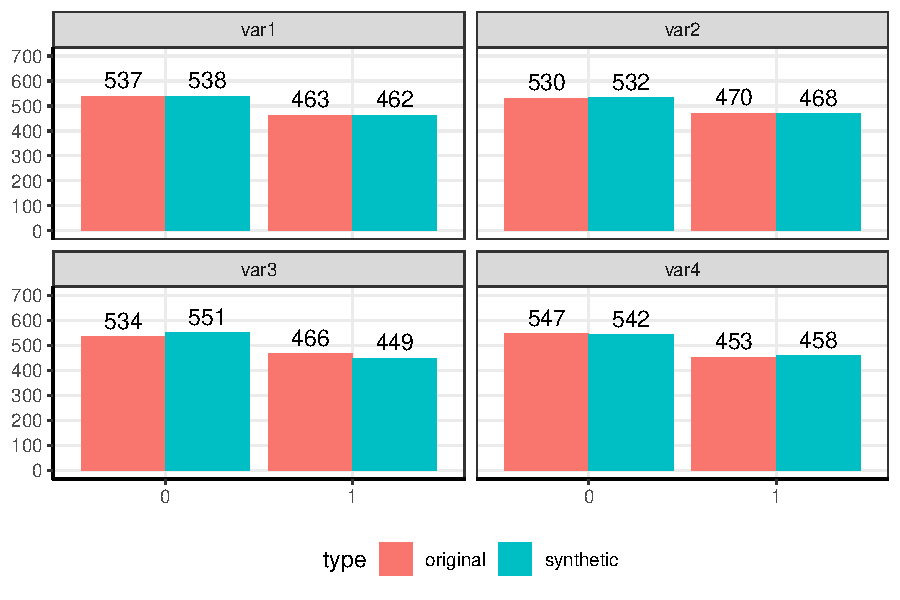
\includegraphics[width=\textwidth]{../graphs/graph_cart_frequency_compare.pdf}
        \caption{Frequency}
        \label{fig:frequency_compare}
    \end{subfigure}
    \hfill
    \begin{subfigure}{0.48\textwidth}
        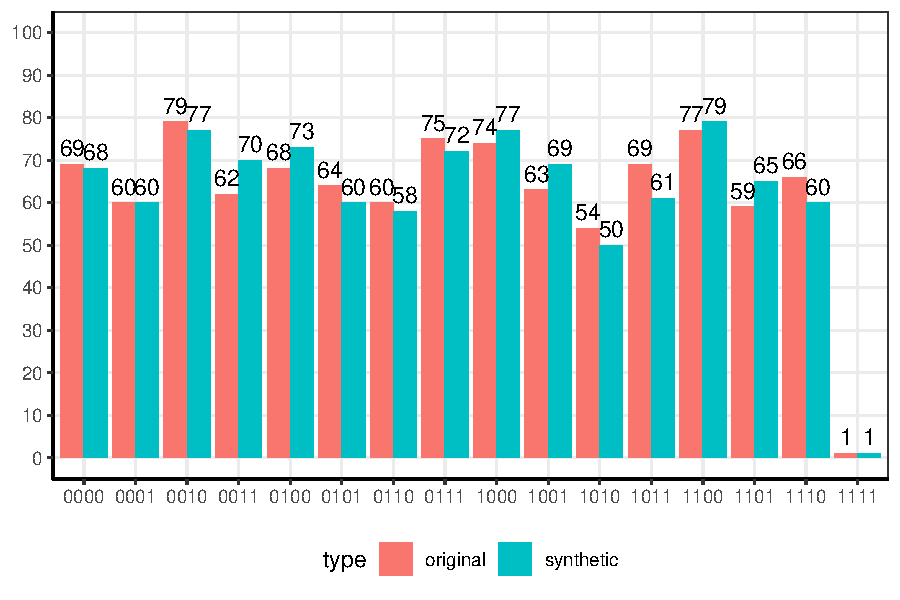
\includegraphics[width=\textwidth]{../graphs/graph_cart_histogram_compare.pdf}
        \caption{Histogram}
        \label{fig:histogram_compare}
    \end{subfigure}
    \label{fig:compare}
\end{figure}

Of 10 synthetic data sets, the frequency of the disclosive record ranges from 0 (2 data sets), 1 (5 data sets), 2 (1 data sets), and 3 (2 data sets).\footnote{For reference, if we created 100 synthetic data sets the frequency of the disclosive record would be similar, ranging from 0 (41 data sets), 1 (38 data sets), 2 (14 data sets), and 3 (7 data sets).}  As a result, regardless of whether one, five, or ten synthetic data sets were released, it would be clear which record was the disclosive record.  As a result, synthetic data from CART models do not protect the unique observation in our simulated data set.  The reason is that in our data with binary categorical data, a record may not be in the synthetic data if it is in the original data, but it can only be in the synthetic data if it is also in the original data.  

\begin{figure}[!h]
    \centering
    \caption{Frequency}
    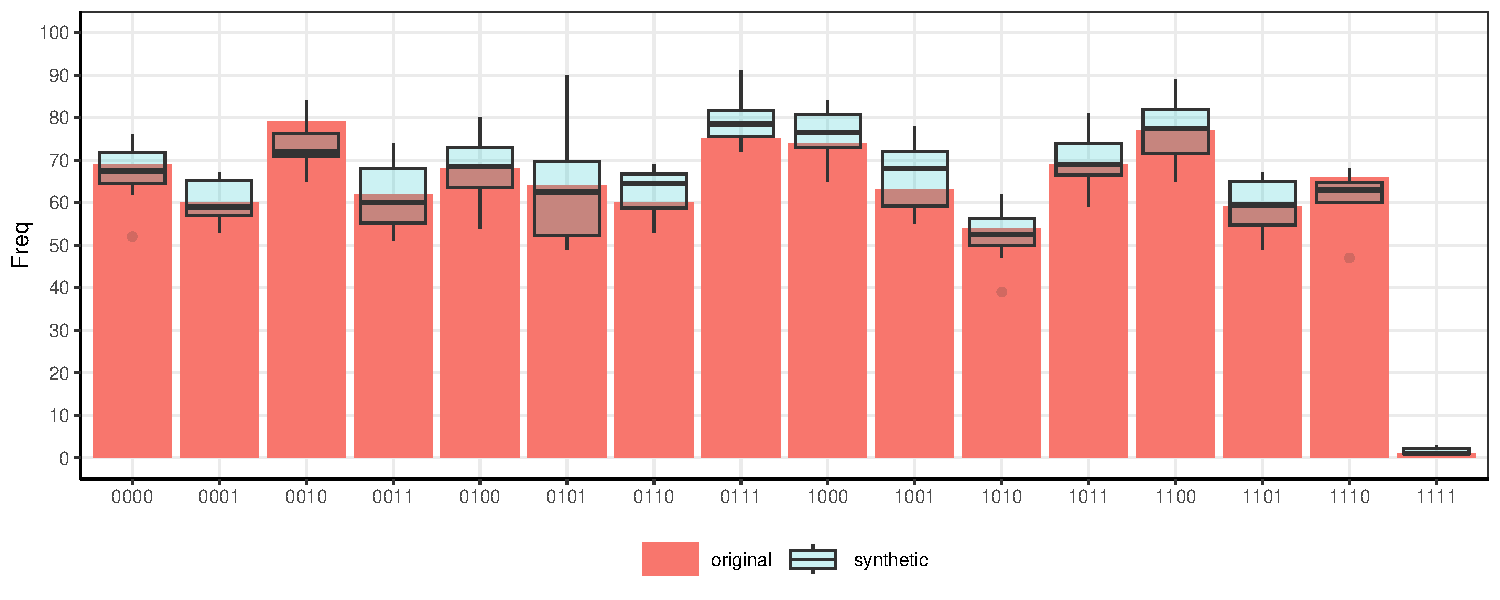
\includegraphics[width=\textwidth]{../graphs/graph_cart_histogram_compare_10.pdf}
    \label{fig:cart_histogram_compare_10}
\end{figure}

\section{The attack}



Figure \ref{fig:attacker_default} illustrates the results of this attack with each attack using 10 synthetic data sets.  In the top left cell, the attacker guesses that the last record in the original data is 0,0,0,0.  They then generate 10 synthetic data sets using a CART-based SDG and compare the histogram to the released synthetic data, as shown in figure \ref{fig:compare}.  Remember, the released synthetic data replicates the single unique record found in the original data (1,1,1,1).  

\begin{figure}[!h]
    \centering
    \caption{Histogram of 16 worlds x 10 synthetic datasets}
    \resizebox{\textwidth}{!}{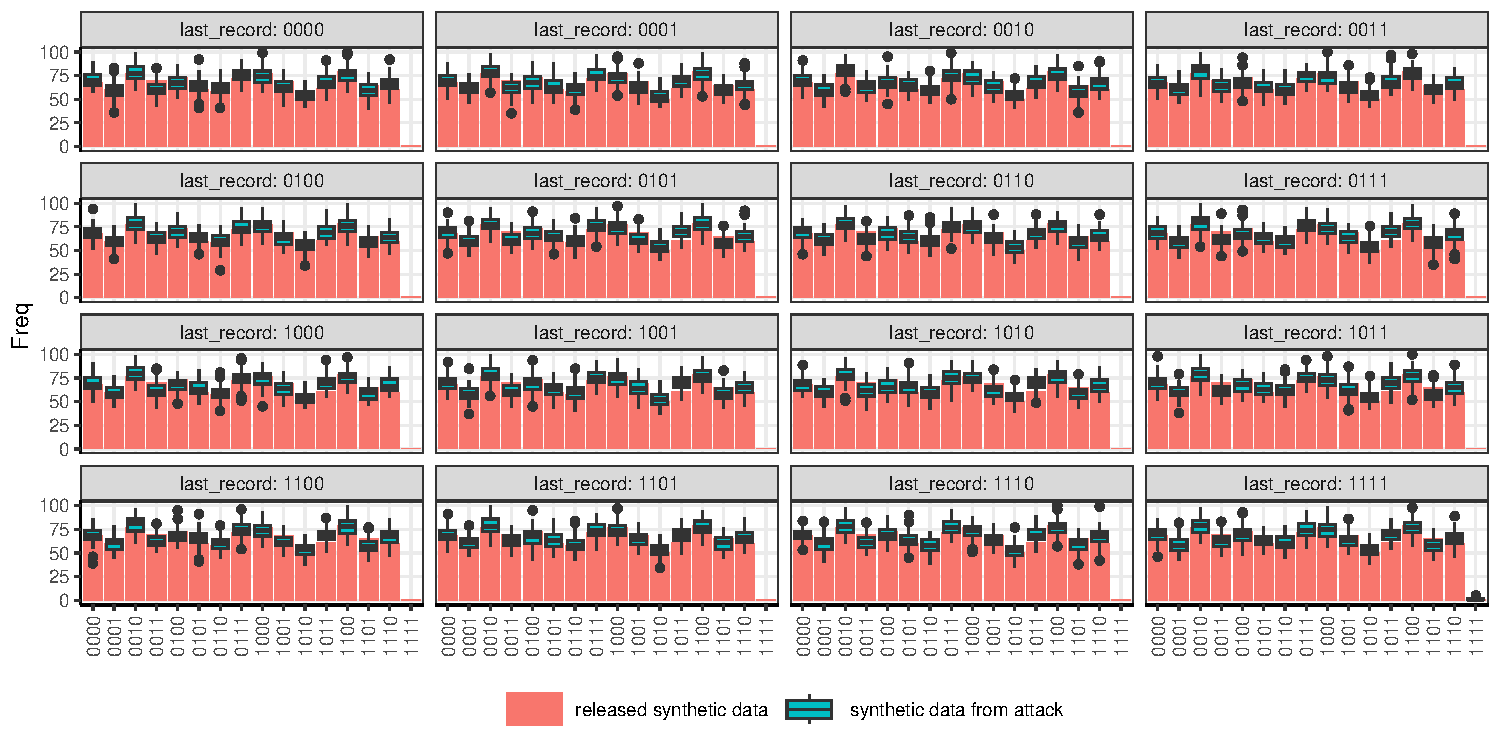
\includegraphics{../graphs/graph_attacker_default.pdf}}
    \label{fig:attacker_default}
\end{figure}

If the attacker guesses that the last record is 0,0,0,0, then they are not able to replicate the single unique record in the synthetic data.  As stated earlier, the reason is that a record may not be in the synthetic data if it is in the original data, but it can only be in the synthetic data if it is also in the original data. 

Next, they update their beliefs about the last record and guess that the last record in the original data is 0,0,0,1.  They then repeat the process as described above.  This is shown in the top row, second column from the left.  Like their first guess, they cannot replicate the released synthetic data.  

The attacker then repeats this process for all 16 possible combinations of the last record.  Finally, if they guess that the last record is 1,1,1,1, then they are able to replicate the released synthetic data, as shown in the bottom, right cell.  The result is a successful attack with confirmation that guess about the values of the last, unique observation is correct.

\section{Privacy}

Our results show that CART can produce synthetic data that is disclosive because it replicates unique records from the original data set without adding sufficient noise.  Other research also indicates that CART-based SDGs can produce synthetic data with high levels of utility because they reproduce a high proportion of the original data \cite{manrique2018bayesian}.  Without denying the fact that achieving high utility by reproducing the original data is a problem, the ability to measure this disclosure is a problem of equal or greater importance.

In table \ref{table:disclosure_risk_1}, the columns display identity and attribute risk measures (the columns) in the original and synthetic data (the rows).  For reference, we replicated table \ref{table:disclosure_risk_1} with 10 synthetic copies from figure \ref{fig:cart_histogram_compare_10}, as shown in table \ref{table:disclosure_risk_10} in the Appendix.  Results are qualitatively similar.  

\begin{table}[]
    \centering
    \caption{Disclosure risk measures}
    % latex table generated in R 4.4.0 by xtable 1.8-4 package
% Tue Jan 14 12:47:47 2025
\begin{tabular}{lrr}
  \toprule
data & identity & attribute \\ 
  \midrule
Original & 0.00 & 0.00 \\ 
  Synthetic & 0.00 & 0.00 \\ 
   \bottomrule
\end{tabular}

    \label{table:disclosure_risk_1}
\end{table}

The identity risk measures are 0 for both the original and synthetic data.  In our data, this is correct because we know that there are multiple combinations of $var1=(0,1)$, $var2=(0,1)$, $var3=(0,1)$.  In other words, the attribute risk correctly identifies that there is zero risk of identity disclosure because there is no unique combination of observations with keys that number three or less variables.

The attribute risk measures are also 0 for both the original or synthetic data.  In our data, this is not correct because we know that when $q=111$, there is a unique record if $t=1$.  

How can it be that there is no attribute disclosure risk when we know there is an attribute disclosure risk?  The answer is that there is only an attribute disclosure risk when $t$ is constant.  In other words, when there is no variation within $q$.  As a result, there is only an attribute disclosure risk when there are 0 copies of the unique record in the synthetic data.  We can see this if we examine the frequency table from 10 synthetic data copies \ref{table:frequency_10_data_sets}, as shown in figure \ref{fig:cart_histogram_compare_10}.  If there is at least 1 unique record, then there is no attribute risk because there are 2 values of $t=(0,1)$ within $q$, but there is an attribute disclosure risk if a synthetic data set is released without a unique record.  This is a problem because the measure incorrectly estimates risk.

In summary, none of the risk measures examined here indicate that there is a problem with disclosure risk in our data.  Therefore, the main issue of concern is that we know there is a disclosure problem (because we created it), but the disclosure risk measures commonly used in the literature do not capture the problem.  

\section{Decreasing privacy risk}

The good news.  We can correct the problem of disclosure risk in synthetic data generated from CART-based SDGs.  If we modify the parameters to avoid overfitting, then the disclosure problem disappears.  There are multiple options to do this.  We use two: increase the minimum number of observations per terminal node to 75 (default is 5) and increase the complexity parameter to 0.05 (default is 1e$^{-8}$), as shown in figure \ref{fig:compare_modified}.  We arrived at these values after doing sensitivity tests, as shown in figure \ref{fig:compare_modified_sensitivity}.  Although values below these do not add enough noise to the data to reduce disclosure risks, these adjustments can reduce disclosure risks.

\begin{figure}[!h]
    \centering
    \caption{Compare original and synthetic data}
    \begin{subfigure}{0.48\textwidth}
        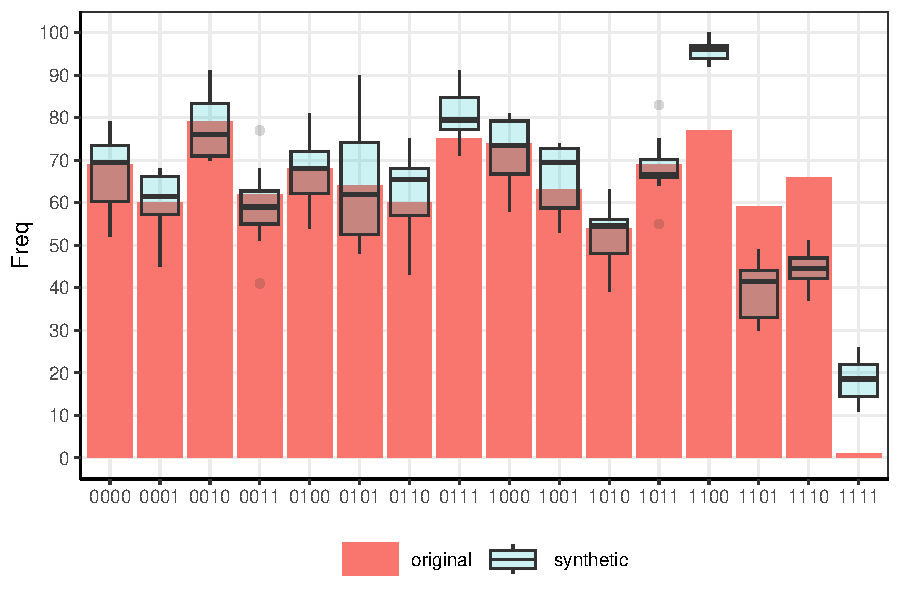
\includegraphics[width=\textwidth]{../graphs/graph_cart_modified_mb_histogram_compare_10.pdf}
        \caption{Minimum bucket is 75}
        \label{fig:attacker_modified_mb}
    \end{subfigure}
    \hfill
    \begin{subfigure}{0.48\textwidth}
        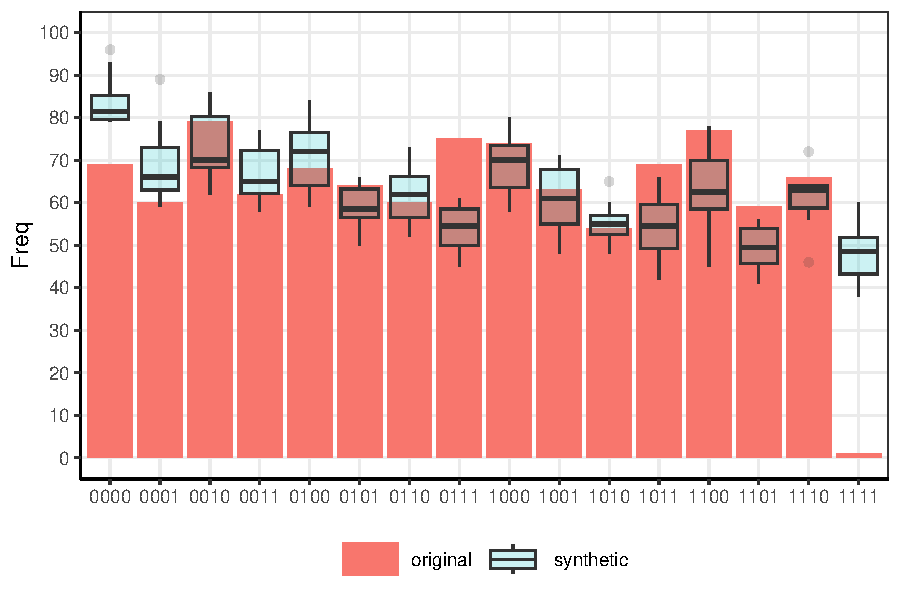
\includegraphics[width=\textwidth]{../graphs/graph_cart_modified_cp_histogram_compare_10.pdf}
        \caption{Complexity parameter is 0.05}
        \label{fig:attacker_modified_cp}
    \end{subfigure}
    \label{fig:compare_modified}
\end{figure}

The bad news.  First, the modified synthetic data may increase privacy, but the sacrifice is lower utility.  Even with 10 synthetic data sets, figure \ref{fig:compare_modified} is less representative of the original data set than figure \ref{fig:cart_histogram_compare_10}.  Second, in an important way, we are voluntarily choosing to decrease utility in order to increase privacy, but remember that no disclosure risk measure indicates that there is a problem.  In a real-world example, we would not know that such sacrifices are justified when risks are not apparent.

For comparison purposes, we have also added noise in the form of $\epsilon$-differential privacy (DP) using the DataSynthesizer package in Python \cite{ping2017datasynthesizer}, as shown in figure \ref{fig:dp_datasynthesizer} in the Appendix.  Similar to figure \ref{fig:compare_modified}, we are able to protect the dislosive record, but only with values of $\epsilon$ equal to or below 0.25, which is far below the common threshold of 1. 

\section{A real world example}

An obvious critique is that the concerns we have raised about privacy measures are demonstrated using a simulated data set that is unlikely to be representative of a real world example.  While we assert that the value of this simulation is to illustrate a sort of `bound' on disclosure risks, we agree with the critique.  In this section, we will demonstrate that the same problems exist in real world data.

Following the authors of Synthpop \cite{raab2024practical}, we rely on data from Social Diagnosis 2011 (SD2011).  In their paper, they generate 5 synthetic data sets to illustrate their method for measuring attribute disclosure by identifying values in the target variable \texttt{depress} from keys: \texttt{sex} \texttt{age} \texttt{region} \texttt{placesize}.  As described above, their preferred measure of attribute disclosure risk (DiSCO) is the set of records in the synthetic data with a constant target ($t$) for the a set of keys ($q$).  In other words, there is no variation in $t$ within $q$.  In their example, attribute risk is about 9\%  (as shown in the table \ref{tab:attribute_risk_sd2011} appendix).  

To illustrate why it is a problem to measure attribute disclosure as the set of records with constant $t$ within $q$, we set $t$ as constant for all observations in all 5 synthetic data sets.  0 was chosen because it is the most frequent value in the variable \texttt{depress} (22\% of all records).  By definition, this reduces attribute disclosure risk.  However, according to the measure of attribute disclosure risk used by the package, the risk increased to around 15\%.

We note that this problem is already understood and described by the package authors \cite{raab2024practical}.  They provide a parameter where a user may check for a target where a high proportion of records have one level (\texttt{check\_1way}).  However, the problem is not the package, the problem is the definition.

In this exercise, we demonstrated a flaw in the measure of attribute disclosure risk using real world data.  The key idea is that we know we reduced risk because we modified the synthetic data by setting a uniform value for the target variable: \texttt{depress} = 0.  Therefore, relative to the original data where there is more risk, risk in the modified data is lower, by definition.  If the measure correctly measured risk, then the risk measure should decline.  Instead, risk is larger in the modified data.  This is not correct.

\section{Conclusion}

In this study, we use a low-dimensional simulated data set with 1.000 observations, four binary variables, and one disclosive record to demonstrate three ideas.  First, CART-based synthetic data generators with default parameters create synthetic data with high levels of utility that reproduce the original data but do not provide protection for the dislosive record.  Therefore, CART-based models are not inherently immune to the utility-privacy trade-off.  Second, not only do common privacy metrics not detect these disclosure risks, but they incorrectly measure disclosure risk by indicating that there is a problem when there is not and indicate that there is not a problem when there is.  Finally, it is possible to increase protection by adding noise to the synthetic data with simple adjustments to the default parameters, but the cost is to reduce utility.  The question is why one would reduce utility if there is no indication there was a disclosure problem?  Given these results, it is important for users interested in reducing disclosure risk to better understand not only how SDGs generate synthetic data, but also how common privacy measures work.  There is no one size fits all solution. 

% \begin{credits}
\subsubsection{\ackname} This work was supported by a grant from the German Federal Ministry of Education and Research (grant number 16KISA096) with funding from the European Union—NextGenerationEU.  Reproducible files are located here: \url{https://github.com/jonlatner/KEM\_GAN/tree/main/latner/projects/simulation}

\subsubsection{Disclosure of Interest} The authors have no competing interests to declare that are relevant to the content of this article.
% \end{credits}

%%%%%%%%%%%%%%%%%%%%%%%%%%%%%%%%
% Bibliography
%%%%%%%%%%%%%%%%%%%%%%%%%%%%%%%%
\bibliographystyle{splncs04}
\bibliography{references}

%%%%%%%%%%%%%%%%%%%%%%%%%%%%%%%%
% Appendix
%%%%%%%%%%%%%%%%%%%%%%%%%%%%%%%%
\clearpage
\appendix
\section{Appendix}\label{appendix}
\setcounter{figure}{0}    
\setcounter{table}{0}    
\renewcommand*\thetable{\Alph{section}.\arabic{table}}
\renewcommand*\thefigure{\Alph{section}.\arabic{figure}}
\renewcommand{\theHfigure}{\Alph{section}.\arabic{table}}
\renewcommand{\theHtable}{\Alph{section}.\arabic{figure}}

\begin{table}[]
    \centering
    \caption{Disclosure risk measures from 10 synthetic data sets}
    \rowcolors{1}{white}{lightgray}
    % latex table generated in R 4.5.0 by xtable 1.8-4 package
% Wed Aug 13 15:48:18 2025
\begin{tabular}{lrr}
  \toprule
Data & Identity Risk ($repU$) & Attribute Risk ($DiSCO$) \\ 
  \midrule
Original & 0.00 & 0.00 \\ 
  Synthetic 1 & 0.00 & 0.00 \\ 
  Synthetic 2 & 0.00 & 6.60 \\ 
  Synthetic 3 & 0.00 & 0.00 \\ 
  Synthetic 4 & 0.00 & 0.00 \\ 
  Synthetic 5 & 0.00 & 0.00 \\ 
  Synthetic 6 & 0.00 & 0.00 \\ 
  Synthetic 7 & 0.00 & 0.00 \\ 
  Synthetic 8 & 0.00 & 6.60 \\ 
  Synthetic 9 & 0.00 & 0.00 \\ 
  Synthetic 10 & 0.00 & 0.00 \\ 
  Average & 0.00 & 1.32 \\ 
   \bottomrule
\end{tabular}

    \label{table:disclosure_risk_10}
\end{table}

\begin{table}[]
    \centering
    \caption{Frequency statistics for original and synthetic data}
    \rowcolors{1}{white}{lightgray}
    % \resizebox{.95\textwidth}{!}{% latex table generated in R 4.4.0 by xtable 1.8-4 package
% Mon Dec 16 16:27:40 2024
\begin{tabular}{lrrrrrrrrrrr}
  \toprule
   & \multicolumn{1}{l}{Original} & \multicolumn{10}{c}{Synthetic Data} \\ \cmidrule(lr){3-12}
 Combine & 0 & 1 & 2 & 3 & 4 & 5 & 6 & 7 & 8 & 9 & 10 \\ 
 \midrule
0000 & 69 & 68 & 66 & 71 & 73 & 76 & 62 & 72 & 52 & 64 & 67 \\ 
  0001 & 60 & 60 & 53 & 57 & 56 & 58 & 60 & 67 & 67 & 57 & 67 \\ 
  0010 & 79 & 77 & 71 & 73 & 71 & 71 & 84 & 65 & 70 & 77 & 74 \\ 
  0011 & 62 & 70 & 51 & 56 & 68 & 63 & 55 & 74 & 57 & 68 & 52 \\ 
  0100 & 68 & 73 & 63 & 80 & 54 & 61 & 79 & 65 & 73 & 66 & 71 \\ 
  0101 & 64 & 60 & 77 & 49 & 66 & 52 & 90 & 52 & 53 & 65 & 71 \\ 
  0110 & 60 & 58 & 68 & 66 & 61 & 69 & 56 & 67 & 65 & 64 & 53 \\ 
  0111 & 75 & 72 & 91 & 86 & 81 & 80 & 77 & 82 & 77 & 75 & 72 \\ 
  1000 & 74 & 77 & 84 & 80 & 73 & 70 & 81 & 82 & 65 & 76 & 73 \\ 
  1001 & 63 & 69 & 66 & 57 & 68 & 73 & 56 & 68 & 75 & 78 & 55 \\ 
  1010 & 54 & 50 & 54 & 57 & 51 & 47 & 50 & 39 & 62 & 58 & 54 \\ 
  1011 & 69 & 61 & 59 & 77 & 71 & 66 & 69 & 75 & 69 & 68 & 81 \\ 
  1100 & 77 & 79 & 77 & 76 & 83 & 78 & 66 & 65 & 88 & 70 & 89 \\ 
  1101 & 59 & 65 & 52 & 54 & 57 & 66 & 67 & 59 & 65 & 49 & 60 \\ 
  1110 & 66 & 60 & 68 & 60 & 64 & 68 & 47 & 65 & 62 & 64 & 60 \\ 
  1111 & 1 & 1 & 0 & 1 & 3 & 2 & 1 & 3 & 0 & 1 & 1 \\ 
   \bottomrule
\end{tabular}
}
    % latex table generated in R 4.4.0 by xtable 1.8-4 package
% Mon Dec 16 16:27:40 2024
\begin{tabular}{lrrrrrrrrrrr}
  \toprule
   & \multicolumn{1}{l}{Original} & \multicolumn{10}{c}{Synthetic Data} \\ \cmidrule(lr){3-12}
 Combine & 0 & 1 & 2 & 3 & 4 & 5 & 6 & 7 & 8 & 9 & 10 \\ 
 \midrule
0000 & 69 & 68 & 66 & 71 & 73 & 76 & 62 & 72 & 52 & 64 & 67 \\ 
  0001 & 60 & 60 & 53 & 57 & 56 & 58 & 60 & 67 & 67 & 57 & 67 \\ 
  0010 & 79 & 77 & 71 & 73 & 71 & 71 & 84 & 65 & 70 & 77 & 74 \\ 
  0011 & 62 & 70 & 51 & 56 & 68 & 63 & 55 & 74 & 57 & 68 & 52 \\ 
  0100 & 68 & 73 & 63 & 80 & 54 & 61 & 79 & 65 & 73 & 66 & 71 \\ 
  0101 & 64 & 60 & 77 & 49 & 66 & 52 & 90 & 52 & 53 & 65 & 71 \\ 
  0110 & 60 & 58 & 68 & 66 & 61 & 69 & 56 & 67 & 65 & 64 & 53 \\ 
  0111 & 75 & 72 & 91 & 86 & 81 & 80 & 77 & 82 & 77 & 75 & 72 \\ 
  1000 & 74 & 77 & 84 & 80 & 73 & 70 & 81 & 82 & 65 & 76 & 73 \\ 
  1001 & 63 & 69 & 66 & 57 & 68 & 73 & 56 & 68 & 75 & 78 & 55 \\ 
  1010 & 54 & 50 & 54 & 57 & 51 & 47 & 50 & 39 & 62 & 58 & 54 \\ 
  1011 & 69 & 61 & 59 & 77 & 71 & 66 & 69 & 75 & 69 & 68 & 81 \\ 
  1100 & 77 & 79 & 77 & 76 & 83 & 78 & 66 & 65 & 88 & 70 & 89 \\ 
  1101 & 59 & 65 & 52 & 54 & 57 & 66 & 67 & 59 & 65 & 49 & 60 \\ 
  1110 & 66 & 60 & 68 & 60 & 64 & 68 & 47 & 65 & 62 & 64 & 60 \\ 
  1111 & 1 & 1 & 0 & 1 & 3 & 2 & 1 & 3 & 0 & 1 & 1 \\ 
   \bottomrule
\end{tabular}

    \label{table:frequency_10_data_sets}
\end{table}


\begin{figure}[!h]
    \centering
    \caption{Compare original and synthetic data with different hyperparameters}
    \begin{subfigure}{0.9\textwidth}
        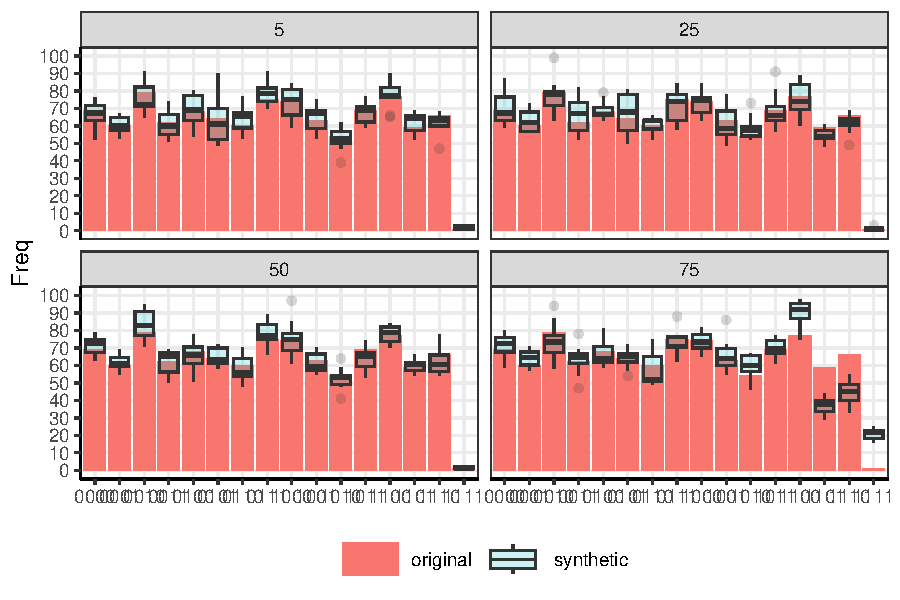
\includegraphics[width=\textwidth]{../graphs/graph_cart_modified_mb_histogram_compare_10_v2.pdf}
        \caption{Minimum bucket (default is 5)}
        \label{fig:attacker_modified_mb_sensitivity}
    \end{subfigure}
    \hfill
    \begin{subfigure}{0.9\textwidth}
        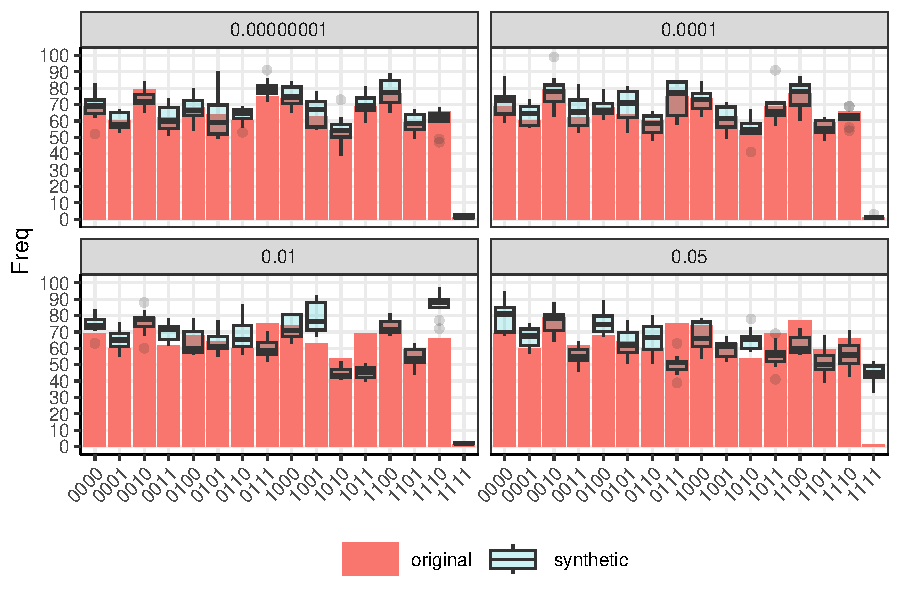
\includegraphics[width=\textwidth]{../graphs/graph_cart_modified_cp_histogram_compare_10_v2.pdf}
        \caption{Complexity parameter (default is 10$^{-8}$)}
        \label{fig:attacker_modified_cp_sensitivity}
    \end{subfigure}
    \label{fig:compare_modified_sensitivity}
\end{figure}


\begin{figure}[!h]
    \centering
    \caption{Datasynthesizer with DP}
    \resizebox{\textwidth}{!}{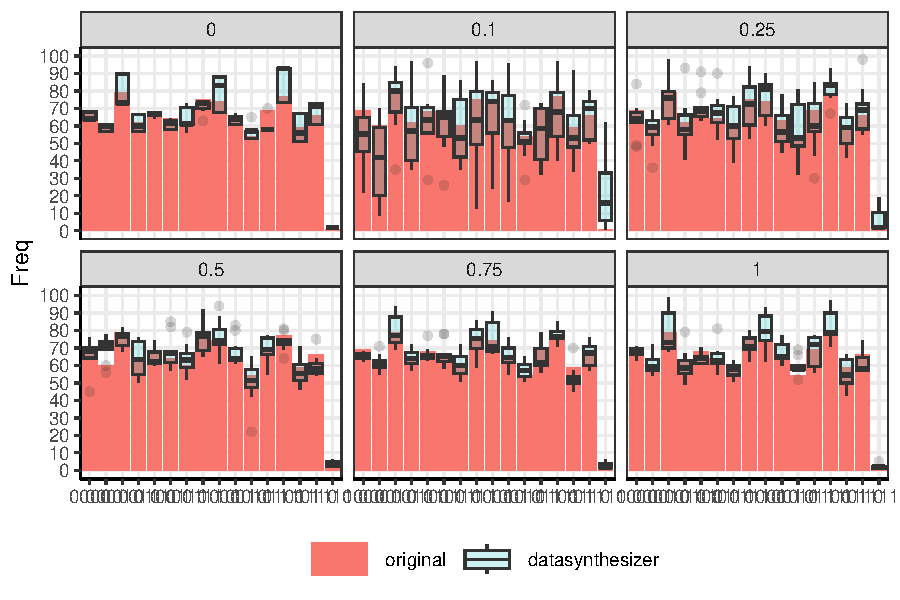
\includegraphics{../graphs/graph_dp_datasynthesizer_compare_histogram_10.pdf}}
    \label{fig:dp_datasynthesizer}
\end{figure}

\begin{table}[]
    \caption{SD2011}
    \label{tab:attribute_risk_sd2011}
    \centering
    \caption{Attribute disclosure measures for \texttt{depress} from keys: \texttt{sex} \texttt{age} \texttt{region} \texttt{placesize}}
    % \rowcolors{1}{white}{lightgray}
    % latex table generated in R 4.4.0 by xtable 1.8-4 package
% Thu Feb 27 14:39:11 2025
\begin{tabular}{lrrrr}
   
\toprule & 
\multicolumn{2}{l}{Identity risk} &
\multicolumn{2}{l}{Attribute risk}
\\  
 
\cmidrule(lr){2-3}
\cmidrule(lr){4-5}
 
Data & Raab et al., 2024 & Modified & Raab et al., 2024 & Modified
\\ 

\midrule
Original data & 48.38 & 48.38 & 53.30 & 53.30 \\ 
  Synthetic 1 & 14.82 & 14.82 & 8.96 & 14.74 \\ 
  Synthetic 2 & 14.20 & 14.20 & 9.90 & 14.82 \\ 
  Synthetic 3 & 15.16 & 15.16 & 10.46 & 14.94 \\ 
  Synthetic 4 & 14.12 & 14.12 & 9.68 & 14.50 \\ 
  Synthetic 5 & 14.30 & 14.30 & 8.88 & 14.66 \\ 
  Average & 14.52 & 14.52 & 9.58 & 14.73 \\ 
   \bottomrule \\[-1.8ex] \multicolumn{5}{p{4in}}{Note: Modified indicates that values of \texttt{depress}=0  in synthetic data} 
\end{tabular}

\end{table}

\end{document}
